\nolinenumbers
\section*{Supplemental Materials and Methods}

\subsection*{Characteristic transcription and translation parameters.}
We used literature based transcription and translation parameters to establish the characteristic synthesis and degradation rates for both mRNA and protein.
We estimated values for the rate parameters from the Bionumbers database \citep{Milo:2010aa}. These parameters were then used for all gene
expression calculations:

\lstset{basicstyle=\tiny,style=myCustomMatlabStyle}
\begin{lstlisting}
-------------------------------------------------------------------
# Description
-------------------------------------------------------------------
cell_diameter = 12                	# \mum
number_of_rnapII = 75000          	# copies/cells
number_of_ribosome = 1e6          	# copies/cells
mRNA_half_life_TF = 2             	# hrs
protein_half_life = 10            	# hrs
doubling_time 	= 19.5         		# hrs
max_translation_rate = 5          	# aa/sec
max_transcription_rate = 6.0       	# nt/sec
average_transcript_length = 15000 	# nt
average_protein_length = 5000     	# aa
fraction_nucleus = 0.49           	# dimensionless
av_number = 6.02e23               	# number/mol
avg_gene_number = 2               	# number of copies of a gene
-------------------------------------------------------------------

---------------------------------------------------------------------------------------
# Description
---------------------------------------------------------------------------------------
# Calculate the volume (units: L)
V = ((1-fraction_nucleus)*(1/6)*(3.14159)*(hl60_diameter)^3)*(1e-15)

# Calculate the rnapII_concentration and ribosome_concentration (units: nM)
rnapII_concentration = number_of_rnapII*(1/av_number)*(1/V)*1e9
ribosome_concentration = number_of_ribosome*(1/av_number)*(1/V)*1e9

# degradation rate constants (units: hr^-1)
degradation_constant_mRNA = -(1/mRNA_half_life_TF)*log(0.5)
degradation_constant_protein = -(1/protein_half_life)*log(0.5)

# kcats for transcription and translation (units: hr^-1)
kcat_transcription = max_transcription_rate*(3600/average_transcript_length)
kcat_translation = max_translation_rate*(3600/average_protein_length)

# Maximum specific growth rate (units: hr^-1)
maximum_specific_growth_rate = (1/doubling_time)*log(2)

# What is the average gene concentration (units: nM)
avg_gene_concentration = avg_gene_number*(1/av_number)*(1/V)*1e9

# Cell death constant (units: hr^-1)
death_rate_constant = 0.2*maximum_specific_growth_rate

# Saturation constants for translation and transcription (units: nM)
saturation_transcription = 4600*(1/av_number)*(1/V)*1e9
saturation_translation = 100000*(1/av_number)*(1/V)*1e9
---------------------------------------------------------------------------------------

\end{lstlisting}

\subsection*{Estimation and cross-validation of EMT model parameters.}
We used the Pareto Optimal Ensemble Technique (POETs) multiobjective optimization framework in combination with leave-one-out cross-validation to estimate an ensemble of TGF$-\beta$/EMT models.
Cross-validation was used to calculate both training and prediction error during the parameter estimation procedure \citep{kohavi1995study}.
The 41 intracellular protein and mRNA data-sets used for identification were organized into 11 objective functions.
These 11 objective functions were then partitioned, where each partition contained ten training objectives and one validation objective.
POETs integrates standard search strategies e.g., Simulated Annealing (SA) or Pattern Search (PS)
with a Pareto-rank fitness assignment \citep{Song:2010fk,JuPOETs-BioArXiv}.
Denote a candidate parameter set at iteration $i+1$ as $\mathbf{k}_{i+1}$.
The squared error for $\mathbf{k}_{i+1}$ for training set $j$ was defined as:
\begin{equation}\label{eqn_cost2}
	E_{j}(\mathbf{k}) = \sum_{i=1}^{\mathcal{T}_{j}}\biggl(\hat{\mathcal{M}}_{ij}-\hat{y}_{ij}(\mathbf{k})\biggr)^2
\end{equation}
The symbol $\hat{\mathcal{M}}_{ij}$ denotes scaled experimental observations (from training set $j$) while $\hat{y}_{ij}$ denotes the scaled simulation output (from training set $j$).
The quantity $i$ denotes the sampled time-index and $\mathcal{T}_{j}$ denotes the number of time points for experiment $j$.
In this study, the experimental data used for model training was typically the band intensity from Western or Northern blots.
Band intensity was estimated using the ImageJ software package \citep{IMAGEJ}.
The scaled measurement for species $x$ at time $i=\{t_{1},t_{2},..,t_{n}\}$ in condition $j$ is given by:
\begin{equation}\label{norm_exp_data}
\hat{\mathcal{M}}_{ij} = \frac{\mathcal{M}_{ij} - \min_{i}\mathcal{M}_{ij}}{\max_{i}{\mathcal{M}_{ij}}-\min_{i}{\mathcal{M}_{ij}}}
\end{equation}
Under this scaling, the lowest intensity band equaled zero while the highest intensity band equaled one.
A similar scaling was defined for the simulation output. By doing this scaling, we trained the model on the relative change in blot intensity, over conditions or time (depending upon the experiment). Thus, when using multiple data sets (possibly from different sources) that were qualitatively similar but quantitatively different e.g., slightly different blot intensities over time or condition, we captured the underlying trends in the scaled data.
JuPOETs is free or charge, open source and available for download under an MIT software license from http://www.varnerlab.org.
Details of the JuPOETs implementation, including example codes are presented in Bassen et al., \citep{JuPOETs-BioArXiv}.

% Additionally, we applied a universal convention of identifying the no expression case as protein value below $<$10$^{-3}$. This is similar to previously published models from our lab. In our studies, Figure 2 identifies experimental data extracted from published Western blots and our simulation results. It is clear from these that 1) the training data included a variety of Western blot data treatments that were effectively zero, and 2) our simulations matched the training data virtually perfectly over time and across multiple biological species. These results validate the power of our simulation scheme, which necessarily includes numerical interpretations of zero. In our Supplemental Figure S9, we present the raw concentrations of our simulations (previously validated from the training data) over hundreds of parameter ensembles, with no “zero” threshold applied.  While these values do not have a threshold, we only interpret values below 10$^{-3}$ equivalent to zero. Likewise, our robustness coefficients (Figure 3) (which represent the ratio of integrated areas of the treatment effect over the baseline effect) identify no difference in model output for vimentin (or e-cadherin for that matter) less than 10$^{-3}$, confirming this interpretation.

\begin{figure}
	\center
	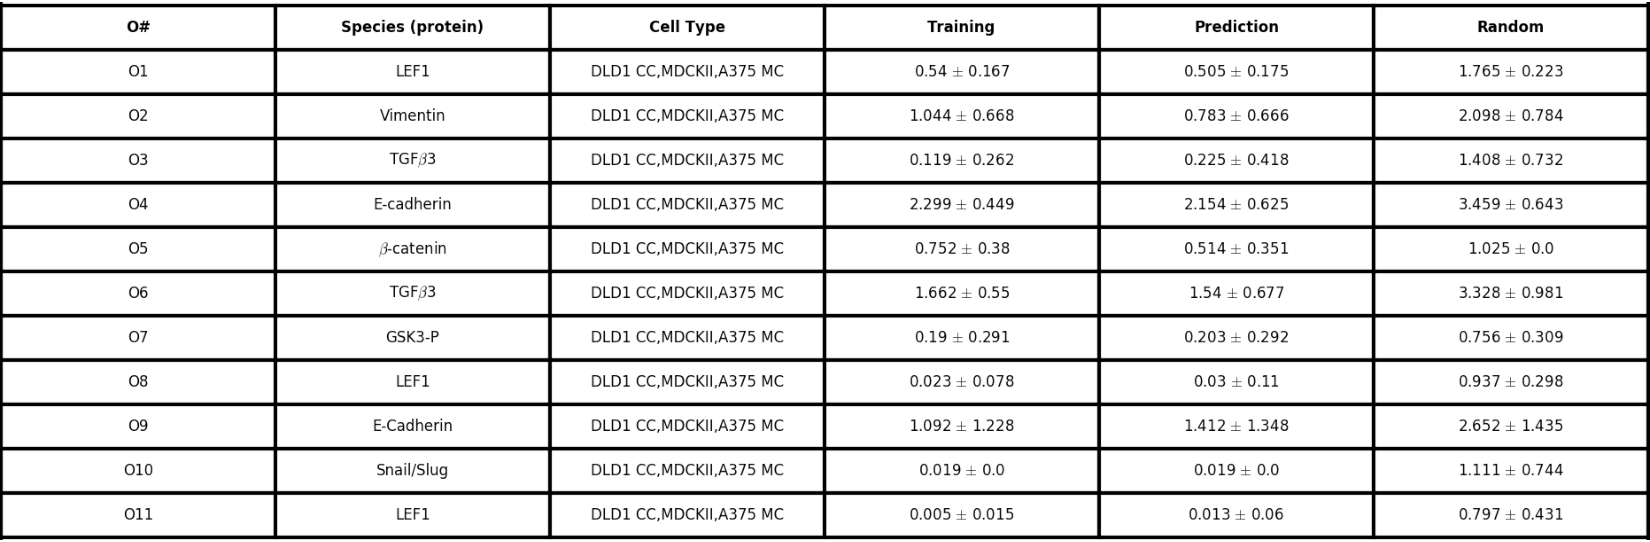
\includegraphics [width=1.0\linewidth] {./figs/Fig-Supplemental-Error-Table.pdf}
	\caption{Training and prediction values as a function of condition for the 11 TGF-$\beta$ objective functions versus a random parameter control.}\label{fg:ObjTable}
\end{figure}

% We computed the Pareto rank of $\mathbf{k}_{i+1}$ by comparing the simulation error at iteration $i+1$ against an archive of accepted parameter sets $\mathbf{K}_{i}$.
% We used the Fonseca and Fleming ranking scheme \cite{fonseca1993genetic} to estimate the number of parameter sets in the archive that dominate
% $\mathbf{k}_{i+1}$. Parameter sets with increasing rank were progressively further away from the optimal trade-off surface.
% The parameter set $\mathbf{k}_{i+1}$ was accepted or rejected by POETs with probability $\mathcal{P}\left(\mathbf{k}_{i+1}\right)$:
% \begin{equation}\label{eqn_costMOSA}
% \mathcal{P}(\mathbf{k}_{i+1}) \equiv \exp{\{-rank\left(\mathbf{k}_{i+1} \mid \mathbf{K}_{i} \right)/T\}}
% \end{equation}
% where $T$ is the annealing temperature and $rank\left(\mathbf{k}_{i+1} \mid \mathbf{K}_{i} \right)$ denotes the Pareto rank for $\mathbf{k}_{i+1}$.
% The annealing temperature was discretized into 10 quanta between $T_{o}$ and $T_{f}$ and adjusted according to the schedule
% $T_k = \beta^k T_0$ where $\beta$ was defined as $\left({T_{f}}/{T_{o}}\right)^{1/10}$.
% The initial temperature was $T_{o} = \mathit{n}/log(2)$, where $n = 4$ in this study and the final temperature was $T_{f} = 0.1$.
% The epoch-counter $k$ was incremented after the addition of 100 members to the ensemble.
% Thus, as the ensemble grew, the likelihood of accepting parameter sets with a large Pareto rank decreased.
% To generate parameter diversity, we randomly perturbed each parameter by $\leq\pm25\%$ at iteration of the search.
% In addition, we performed a local pattern search every $q$-iterations to minimize the residual for a single random or the worst performing objective function.
% The local pattern-search algorithm has been described previously \cite{gadkar2003cybernetic}.
% From the 15,000 probable EMT models, we selected N = 1093 models with Pareto rank $\leq{1}$ for subsequent analysis.
% A quick estimate of the set to set correlation showed that we could expect on order 25\% correlation between parameter sets in the ensemble.

% \begin{figure}
% 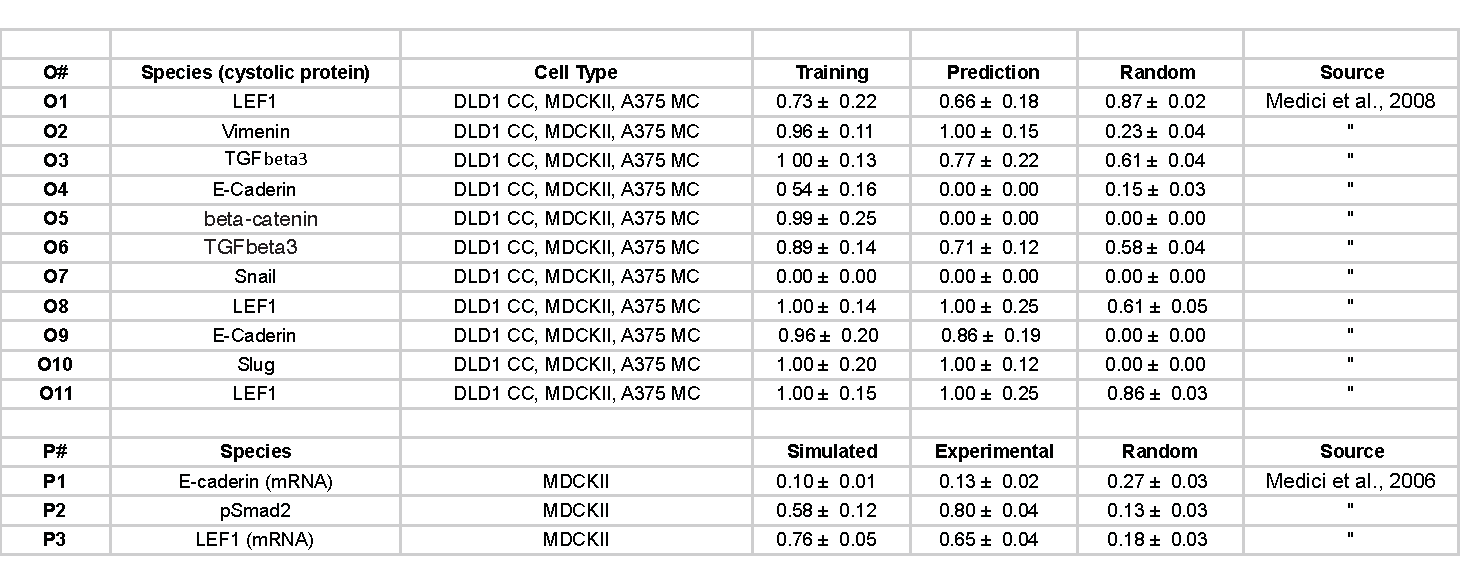
\includegraphics [width=1.0\linewidth] {./figs/Fig-5-Supplemental-ErrorTable.pdf}
% \caption{Training and prediction values for the 11 TGF-$\beta$ objective functions versus a random parameter control.}\label{fig:S5}
% \end{figure}

% \begin{figure}
% 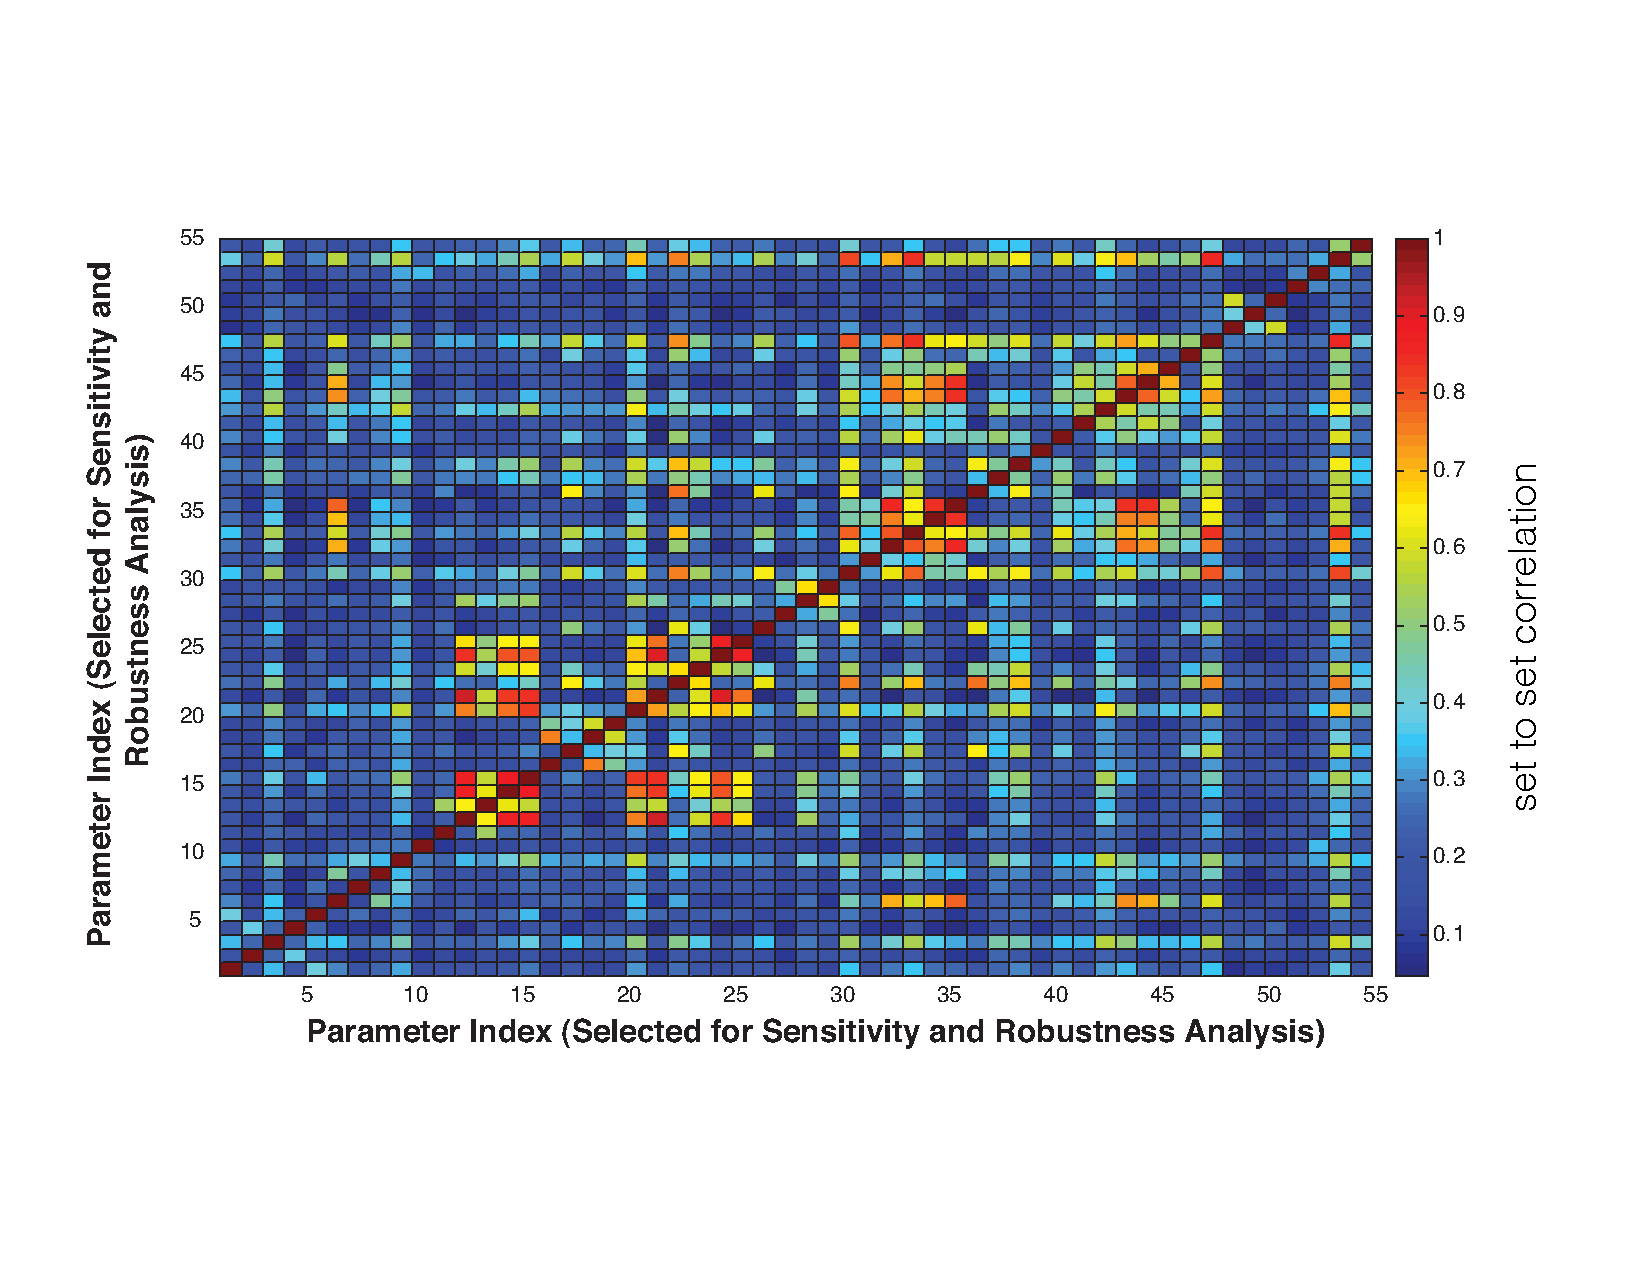
\includegraphics [width=1.0\linewidth] {./figs/Fig-7-Supplemental-Correlation.pdf}
% \caption{Parameter set to set correlation for 55 random parameter sets selected from the ensemble.
% Of the 55 sets selected, the average correlation between sets was less than 25\% for greater than 80\% of the parameter sets.}\label{fig:S7}
% \end{figure}

% \begin{figure}
% 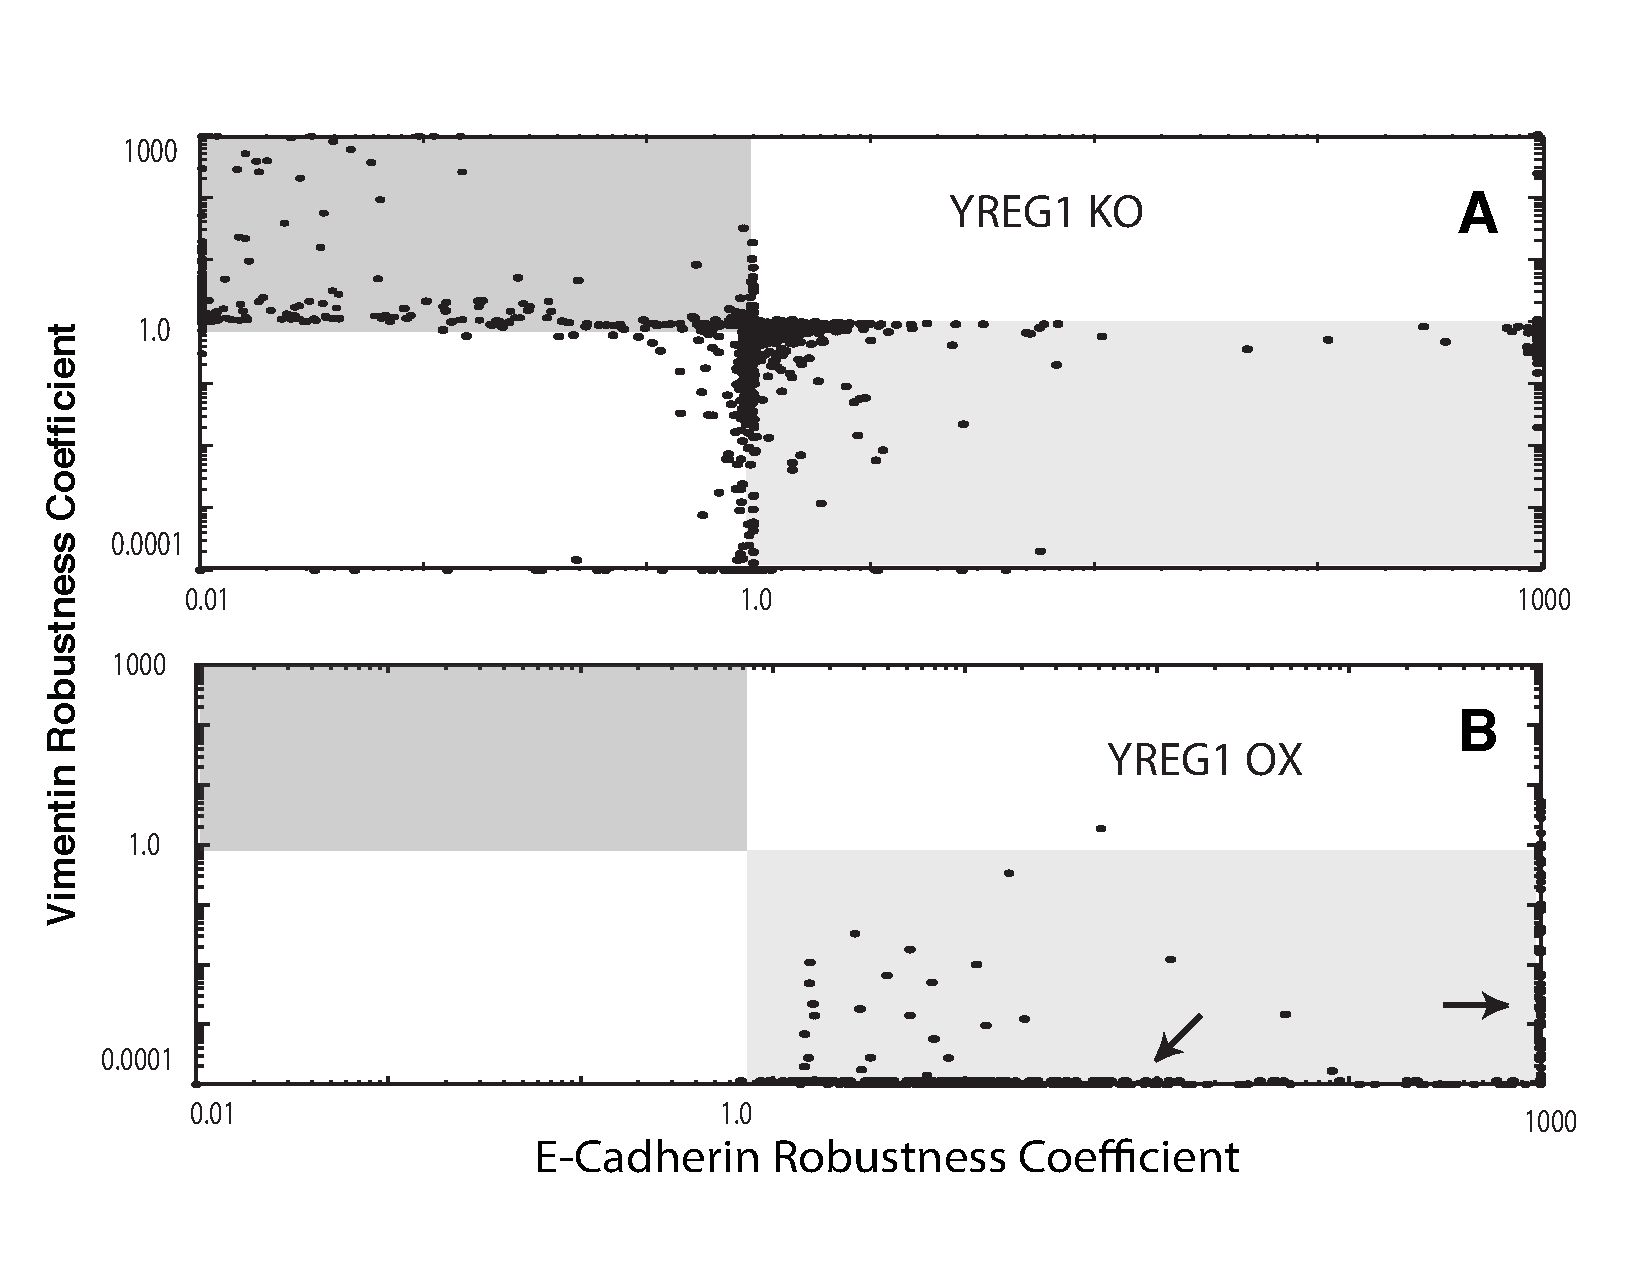
\includegraphics [width=1.0\linewidth] {./figs/Fig-8-Supplemental-YREG1.pdf}
% \caption{Robustness of E-cadherin and Vimentin expression to a knockout (A) and overexpression (B) of the hypothetical regulator 1 (YREG1) protein.
% Robustness coefficients were calculated for each member of the ensemble. Each point represents the response of a single model in the ensemble to either a knockout or
% overexpression of YREG1.}\label{fig:S8}
% \end{figure}

% \begin{figure}
% 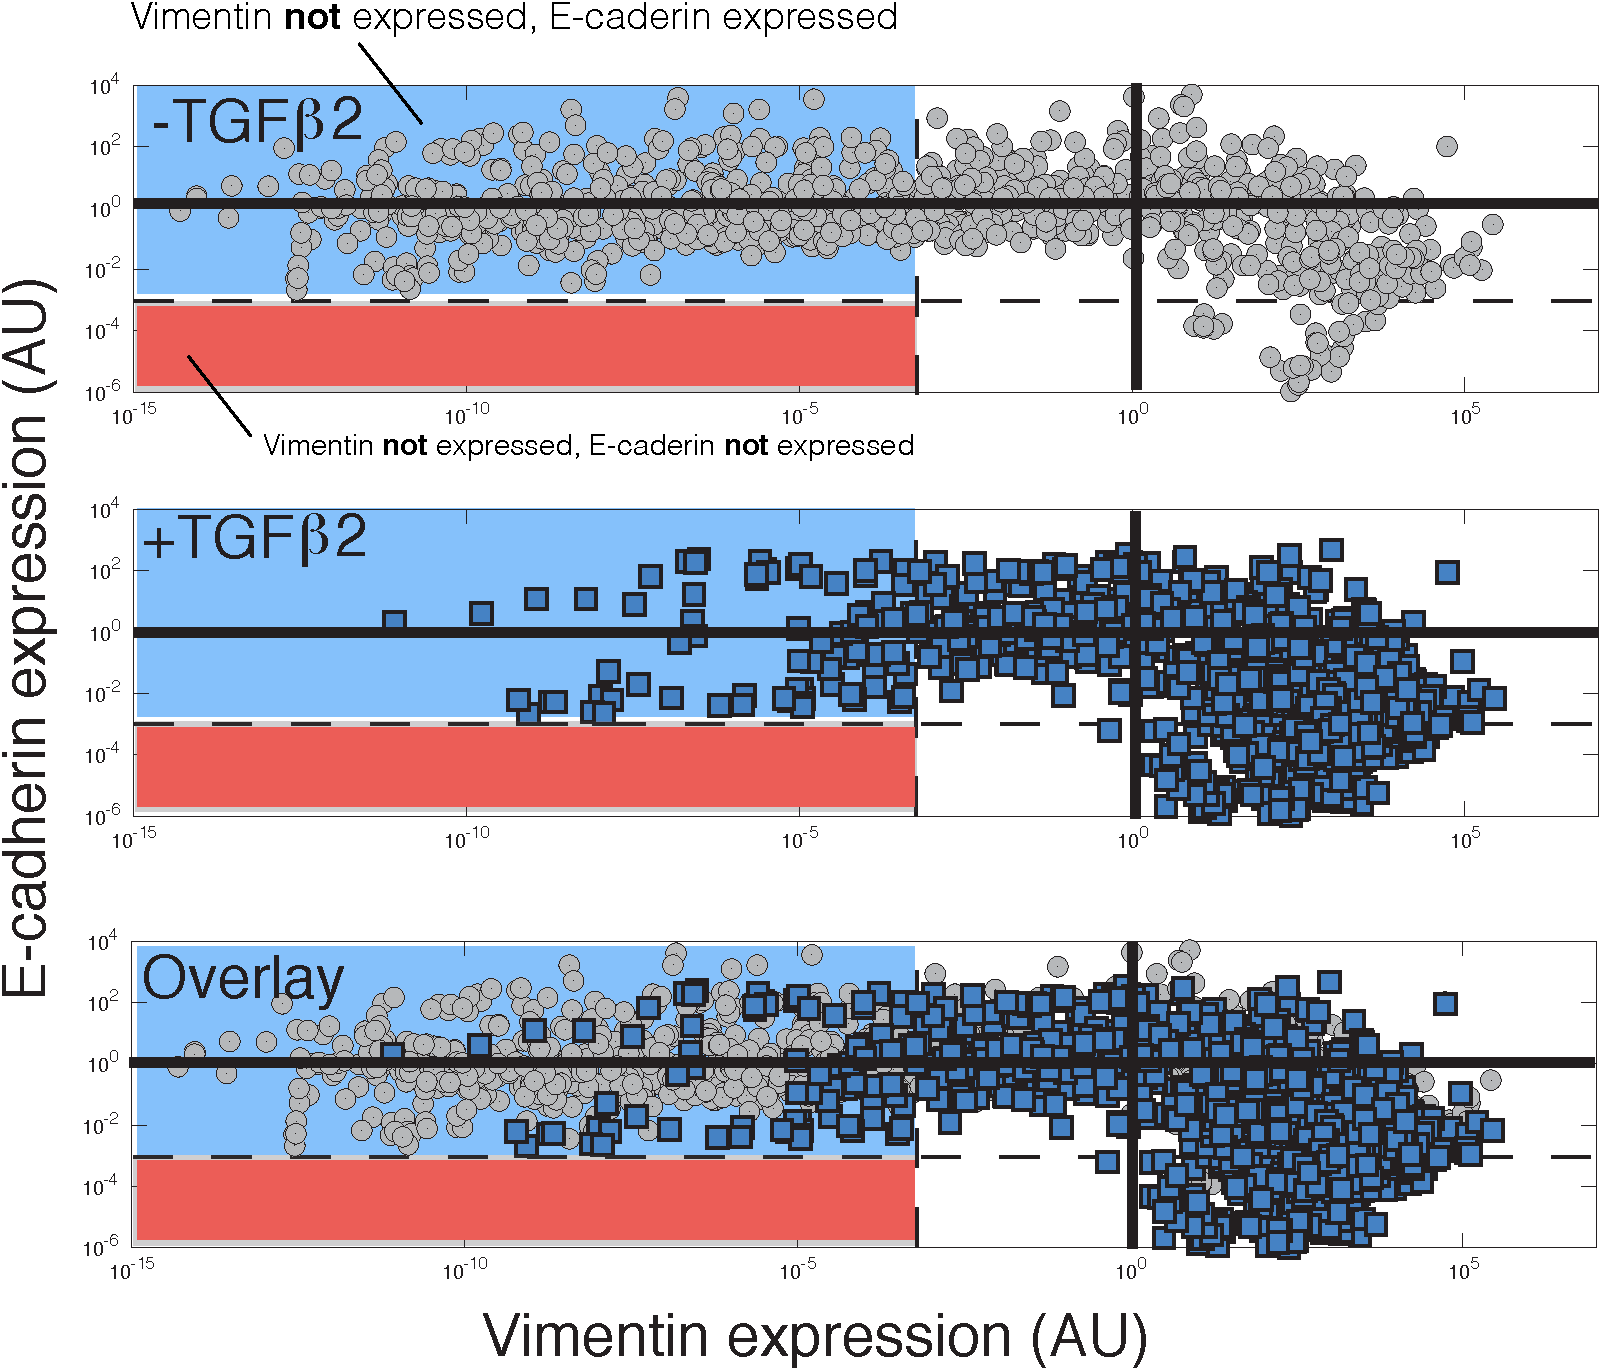
\includegraphics [width=1.0\linewidth] {./figs/Fig-9-Supplemental-RawExpression_v2.pdf}
% \caption{Steady state protein abundance for E-cadherin and Vimentin (AU) as a function of TGF-$\beta$1/2 exposure.
% Top: Overlay of the model population for Vimentin (AU) and E-cadherin (AU) expression in the presence (blue) and absence (gray) of TGF-$\beta$1/2.
% Midddle: Vimentin (AU) and E-cadherin (AU) expression in the absence of TGF-$\beta$1/2 showed exhinibted population heterogenity.
% Bottom: Vimentin (AU) and E-cadherin (AU) expression in the presence of TGF-$\beta$1/2 moved the centriod of the population toward Vimentin (AU) and away from E-cadherin (AU) expression.}\label{fig:S9}
% \end{figure}

% \subsection*{EMT model network architecture.} TGF$\beta$ is a major inducer of EMT in development, fibrosis, and carcinogenesis with different isoforms mediating various effects depending on specific cellular context \cite{Nawshad:2005pi}.
% TGF$\beta$1 was first described as an inducer of EMT in normal mammary epithelial cells \cite{Miettinen1994} and has since been shown to mediate EMT in vitro in a number of different epithelial cells, including renal proximal tubular, DLD1 colon carcinoma, and most recently alveolar epithelial cells \cite{Fan1999, Hales1994,Kasai2005,Willis2005}.
% TGF$\beta$ signaling occurs through the Smad pathway in which signals are transduced by transmembrane serine/threonine kinase type I (ALK5) and type II (TGF$\beta$RII) receptors.
% To increase ligand affinity, betaglycan (TGF$\beta$RIII) can also interact with TGF$\beta$RI,II \cite{Gatza:2010if}.
% Upon TGF$\beta$ stimulation, the receptors are internalized into early endosomes where Smad anchor for receptor activation (SARA) modulates formation of complexes with (R-Smad) Smad2 or Smad3.
% Smad2 and Smad3 are then phosphorylated at serine residues by the type I receptor \cite{Massague:2005qc}.
% Phosphorylation induces their association with (Co-Smad) Smad4 and translocation to the nucleus where they interact with other transcription factors to regulate the transcription of TGF$\beta$ responsive genes, including alpha-smooth muscle actin, collagen1A2, vimentin, fibronectin, and plasminogen activator inhibitor-1 (PAI-1) by interacting with Smad-binding elements \cite{Dennler:2002hl,Derynck:2003fc}.
% To regulate TGF$\beta$ signaling, Smurf2 (a ubiquitin E3 ligase) can become activated to mediate proteasome dependent degradation of Smad2 or bind with Smad 7 to target TGF$\beta$ receptor for degradation \cite{Kavsak2000,Bonni2001}.
%
% \subsubsection*{Cell Type Dependency} Interestingly, differential roles for Smad2 and Smad3 in TGF$\beta$ induced EMT have been demonstrated.
% For example, using primary cells from mice with hepatocyte-specific double knockout of Smad2 and Smad3, it was demonstrated that Smad3 but not Smad2 was required for a key morphological changes and induction of EMT \cite{Ju:2006so}.
% In contrast, using human proximal tubular epithelial cells, increased colony growth factor and decreased E-cadherin were Smad3 dependent, increased MMP-2 was Smad2 dependent, while alpha-smooth muscle actin was dependent on both \cite{Phanish2006}.
% Furthermore, Smad2 signaling has been demonstrated in cancerous lung epithelial A549 cells \cite{Kasai2005}.
% Inhibition of Smad3 signaling decreases the metastatic potential of xenografted breast cancer cell lines \cite{Tian2003,Tian2004}.
% Together, these results suggest that the precise Smad pathway activated may depend on the particular cellular context.
% Regardless, a recent transcriptomic analysis of TGF$\beta$ induced EMT in normal mouse and human epithelial cells using a dominant negative approach demonstrated that Smad signaling was critical for regulation of all tested target genes \cite{Valcourt2005}.
%
% \subsubsection*{Smad-Independent EMT Induction Pathways. }Although less well established than the Smad-dependent pathways in the induction of EMT, there is substantial evidence for TGF$\beta$ activation of Smad-independent signaling in some aspects of this process.
% These include RhoA, MAPK, PI3 kinase, and Notch signaling pathway, which have mostly been studied in-vitro.
% For example, the small GTPase RhoA is involved in TGF$\beta$ induced EMT in a number of cell types including NMuMG mammary epithelial cells and mink lung epithelial (Mv1Lu) cells particularly in the regulation of cytoskeletal and adherens junction rearrangement.
% In addition to its role in cytoskeletal remodeling, Rho has been shown to activate the alpha-smooth muscle promoter during EMT in kidney proximal tubular (LLCPK1) cells \cite{Masszi:2003hb}.
% TGF$\beta$ has been shown to elevate ERK activity in culture models of EMT (human keratinocytes, NMuMG mammary epithelial cells, and mouse cortical tubule epithelial cells) \cite{Zavadil2001,Xie2004,Davies2005}.
% This ERK activity was required for disassembly of adherens junctions and induction of cell motility \cite{Xie2004}.
% Inhibition of ERK blocked these key morphological changes of EMT in mammary gland epithelial cells \cite{Xie2003}.
% Recent studies in MDCKII and DLD1 colon carcinoma cells revealed that TGF$\beta$3 can signal through PI3 kinase.
% Upon activation, PI3 kinase activates molecules such as ILK and AKT, which can phosphorylate and inactivate GSK3$\beta$, a protein that targets both Snail and $\beta$-catenin for degradation through the ubiquitin proteosome pathway \cite{Medici:2008fk}.
% Lastly, there is increasing evidence for a role of Notch pathways in regulating EMT, particularly during development \cite{Nawshad:2005pi}.
% In cardiac cushion EMT, it was found that that Slug is directly up-regulated by Notch in endothelial cells repression of the vascular endothelial cadherin promoter and for promoting migration of transformed endothelial cells.
% In whole, the distinction between Smad-dependent and Smad-independent mechanisms remains difficult to interpret due to the significant cross talk between these pathways.
% In most cases, stimulation of these cooperative pathways provides the context for induction and specification of EMT within a particular tissue/cell type, with Smads representing the dominant pathway, which in some instances may be necessary but not sufficient for induction of full EMT \cite{Zavadil:2005fu}.
%
% \subsubsection*{Master Transcription Regulators}
% Master transcription factors of EMT are thought to be regulated by Snail1 (SNAI1) and Snail2 (SNAI2) (previously known as Snail and Slug, respectively).
% These transcription factors are zinc finger proteins that function as repressors of E-cadherin transcription in cultured epithelial cells \cite{Cano:2000kh}, repression of E-cadherin leads to dissolution of adherens junctions.
% Snail and Slug can be activated by TGF$\beta$ via both Smad-dependent and -independent pathways in a cell type dependent fashion in cultured cells \cite{Peinado2003}.
% Differential expression of Snail and Slug is observed in TGF$\beta$ induced EMT in keratinocytes, renal proximal tubular, and mammary epithelial cells, suggesting that they are regulated in a cell specific.
% Interestingly, key regulatory units of Snail and Slug appear to be regulated by upstream transcription factors AP1 and SP1, respectively.
% Peinado et al. clearly established a necessary role of Snail in mediating TGF$\beta$1 induced EMT in MDCK cells.
% They demonstrated that the Ras-Raf-MEK-ERK-AP1 signaling pathway could up-regulate synthesis of the E-cadherin repressor molecule Snail (directly binds to Snail promoter) \cite{Peinado:2004pt}.
% Likewise, TGF$\beta$1 induced the expression of Slug in both lens and other epithelial cells in vitro.
% The Sp1 binding site in the Slug promoter is largely responsible for TGF$\beta$1 induced Slug expression and upstream of MAPK signaling.
% In addition, the TGF$\beta$1 mediated repression of E-cadherin was significantly inhibited by Slug siRNA \cite{Choi2007}.
%
% \subsubsection*{ERK/MAPK Crosstalk}
% The ERK-MAPK pathway has been shown to modify TGF$\beta$ signaling at multiple levels.
% One way is that the activated Ras pathway inhibits the TGF$\beta$ induced nuclear accumulation of Smad2/3, as seen in epithelial cells \cite{Zhang2009a}.
% ERK kinases have been shown to phosphorylate Smad2 and Smad3 at specific sites in the region linking the MH1 and MH2 domains.
% These sites are separate from the TGF$\beta$ receptor phosphorylation sites which activate Smad nuclear translocation \cite{Massague2003}.
% The effect of interaction between ERKs and Smads is the subject of some controversy, with data suggesting that such an interaction either enhances or inhibits downstream events.
% A hyperactive Ras pathway has been shown to effectively counteract the antiproliferative activity of TGF$\beta$ through attenuation of Smad accumulation in the nucleus \cite{Kretzschmar:1999wb}.
% In contrast, Ras signals strongly cooperated with Smads for invasion of human carcinoma cells \cite{Oft1996}.
% A second way is through transcriptional regulation.
% Recently, it was found that Sp1, via transcriptional induction of Vimentin, cooperates with activated Smad complexes in mesenchymal transition and migration of pancreatic cancer cells upon TGF$\beta$ stimulation \cite{Jungert:2007ri}.
% Likewise, binding sites at the SP1/Smad3 complex was found to regulate the betaglycan receptors \cite{Lopez-Casillas2003}.
% Taken together, multiple levels of cross-talk (both positive and negative) exist within MAPK and TGF$\beta$, and may also be cell type dependent.
%
% \subsection*{Analysis of the signal flow through the EMT architecture.}
% To investigate temporal shifts for key species dominating the EMT response, we calculated the scaled flux through the signaling architecture (Fig. \ref{fg:S1}).
% Three modes of operation were simulated to identify distinct behavioral differences: (a) no TGF-$\beta$2 (-TGF-$\beta$1/2), (b) TGF-$\beta$1/2 stimulation (+TGF-$\beta$2),
% and (c) TGF-$\beta$1/2 stimulation while blocking the autocrine response of TGF-$\beta$3 (+TGF-$\beta$1/2 + TGF-$\beta$3Ab).
% Following TGF-$\beta$1/2 stimulation, AP1/SP1 rapidly stimulates Snail/Slug expression (Fig. \ref{fg:S1}A) within 1 hr.
% During this phase, Snail/Slug repress E-cadherin expression, which in turn reduces the interaction between E-cadherin and $\beta$-catenin, and the accumulation of free cytosolic $\beta$-catenin ensues.
% Conversely, in the presences of a TGF-$\beta$3 neutralizing antibody, membrane bound $\beta$-catenin increased after 10 hrs,
% while low levels of free cytosolic $\beta$-catenin accumulated between 1-5 hrs (Fig. \ref{fg:S2}A,B).  Accumulation of free $\beta$-catenin is critical for complexing with TCF4 to rapidly produce the autocrine response of TGF-$\beta$3 within 1-10 hrs.  Following TGF-$\beta$3 expression, formation and spatial relocation of the Smad complexes occurs in a time dependent manner.  Smad2 is phosphorylated within 1 hr and nuclear localization of the pSmad2/4 complex dramatically increases after 10 hours (Fig. \ref{fg:S1}C).  This timely formation is critical for completion of the EMT process.  At steady state, the E-cadherin complex was maintained at a basal epithelial level with no expression of Vimentin (Fig. \ref{fg:S1}D). During TGF-$\beta$1/2 stimulation, both MAPK and Smad act synergistically to repress the E-cadherin complex within 1 hr.
% This is followed by increase of Vimentin at $\sim$ 1hr, while exponentially increasing around 10 hrs.
% Both species elevate within 1 hr, however the complex does not significantly form until $\sim$ 10 hrs.
% When blocking TGF-$\beta$3, Snail/Slug downregulates the E-cadherin complex between 5-10 hrs,
% but cannot complete the transformation due to the loss of Smad2 phosphorylation (Fig. \ref{fg:S1}D).
%
% \begin{figure}
% 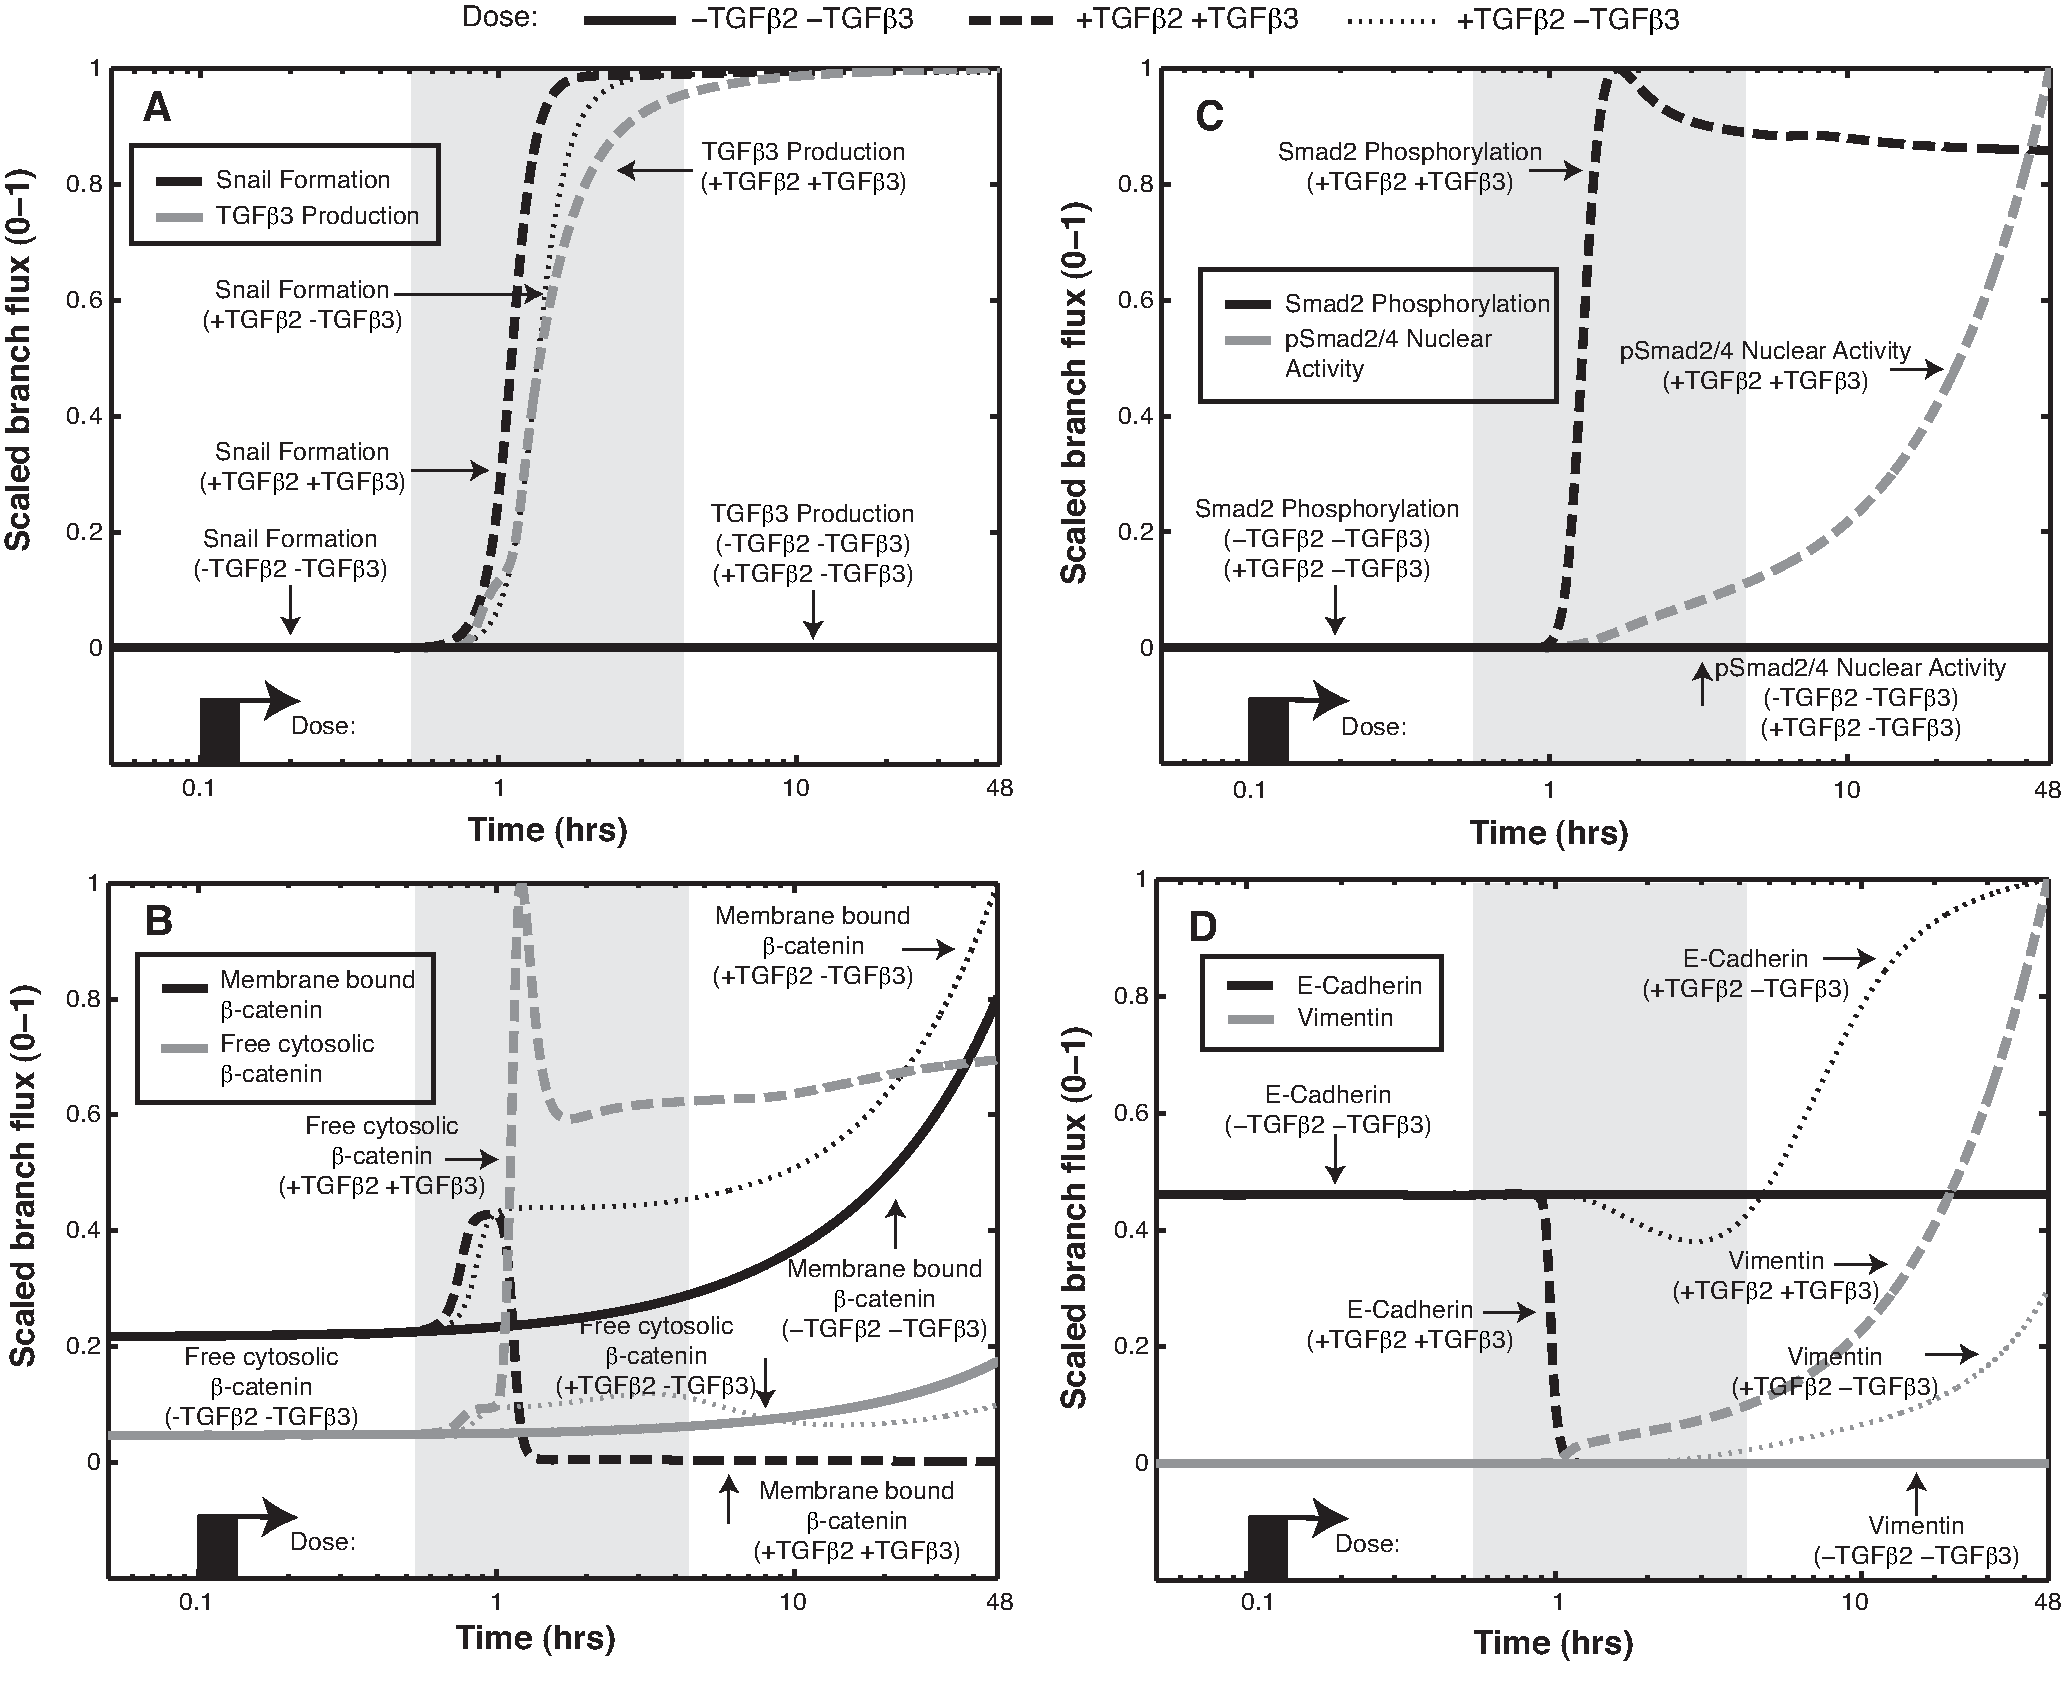
\includegraphics [width=1.0\linewidth] {./figs/Fig-1-Supplemental-FluxAnalysis.pdf}
% \caption{Signal flow analysis of key species at steady state, TGF-$\beta$1/2 stimulation, and blocking the TGF-$\beta$3 autocrine response.
% (A)  The MAPK cascade is directly responsible for rapid expression of Snail and downstream TGF-$\beta$3 formation (1~hrs).
% (B) TGF-$\beta$1/2 reduces  $\beta$-catenin, allowing rapid free-cytosolic $\beta$-catenin to accumulate (1hr).
% Blocking TGF$\beta$3 increases membrane bound $\beta$-catenin (10hr). (C)  TGF-$\beta$3 activates the Smad cascade.
% Nuclear localization of the pSmad2/4 complex (10~hrs) is dependent upon both the phosphorylation of Smad2 (1~hrs) and complexing with Smad4 (5~hrs).
% (D)  TGF-$\beta$1/2 rapidly reduces the E-cadherin complex, while upregulating Vimentin (5-10 hrs).
% Blocking TGF$\beta$3 increases E-cadherin (10~hrs) and Vimentin is significantly reduced.}\label{fg:S1}
% \end{figure}
%
% \begin{figure}
% 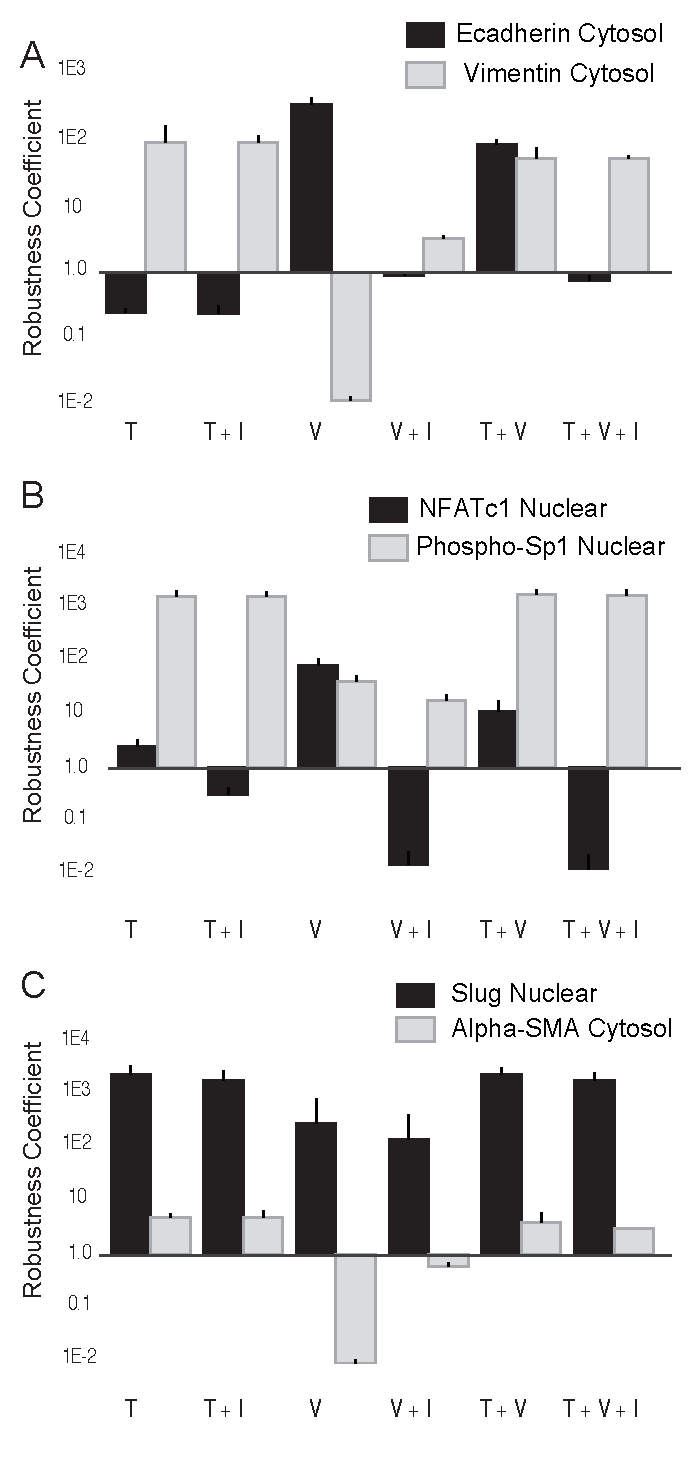
\includegraphics [width=0.5\linewidth] {./figs/Fig-2-Supplemental-Robustness.pdf}
% %\includegraphics [width=1.0\linewidth] {./ManuFigures/Figs/F2.pdf}
% %\epsfig{file=./figures/Figures_EMT_Manuscript/Final/ManuFigures/F2.eps,,width=1.0\textwidth}
% \caption{Robustness analysis for key molecular species at t = 48 hrs for combinations of TGF-$\beta$1/2, VEGF-A and NFATc1 inhibitors. Robustness coefficients for the indicated species were calculated
% for N $\sim{1100}$ ensemble members for 48 hrs following the addition of TGF-$\beta$1/2 (T), TGF-$\beta$1/2 + NFATc1 inhibitor (T + I), VEGF-A (V), VEGF-A + NFATc1 inhibitor (V + I) and TGF-$\beta$1/2 + VEGF-A (T+V) + NFATc1 inhibitor (T + V + I).
% (A) Robustness coefficients for E-cadherin and Vimentin as a function of condition.
% (B) Robustness coefficients for nuclear localized phosphorylated Sp1 and NFATc1 as a function of condition.
% (C) Robustness coefficients for nuclear localized Slug and $\alpha$-smooth muscle actin ($\alpha$-SMA) as a function of condition.
% In each case the error bars denote one-standard deviation of robustness coefficient calculated over the model ensemble.
% C=Control, T=TGF$\beta$2 , V=VEGFA, VI= NFAT inhibitor (VIVIT).}\label{fg:S2}
% \end{figure}


\begin{figure}
\includegraphics [width=1.0\linewidth] {./figs/Fig-3-Supplemental-DLD1.pdf}
\caption{VEGF-A attenuates TGF-$\beta$1/2 to induce phenotype heterogeneity in DLD1.
(A) In DLD1, we found that 5ng/ml of VEGFA increased NFATc1 and E-cadherin gene expression via qPCR and 50ng/ml potentiated this effect at 48 hrs.
(B - C) These findings were confirmed at the protein level via immunofluorescence, as ecadherin levels and nuclear localization of NFATc1 increased.
(D) Treatment with (10ng/ml) TGF$\beta$2 resulted in mesenchymal transformation as measured via qPCR against target genes Slug, ecadherin, vimentin, Sp1, and NFATc1.
(E - F) Immunofluorescence and nuclear localization revealed a strong presence of phospho-Sp1.
(G) Combination of VEGFA (50ng/ml) and TGF$\beta$2 (10ng/ml) treatment resulted in increased Slug, NFATc1, and vimentin expression, while also increasing ecadherin levels compared to control.
(H) Immunofluorescence confirmed these results, as both ecadherin and vimentin levels were elevated.
(I) A significant increase in nuclear localization of both NFATc1 and phospho-Sp1 were also found.
Magnification, 40x. Scale bars: 50$\mu$m.  C=Control, T=TGF$\beta$2 , V=VEGFA, VI=NFAT inhibitor (VIVIT).
Asterisks signify statistical differences from each other according to a one-way ANOVA with Tukey's post hoc (p$\prec$0.05).}\label{fg:S3}
\end{figure}

\begin{figure}
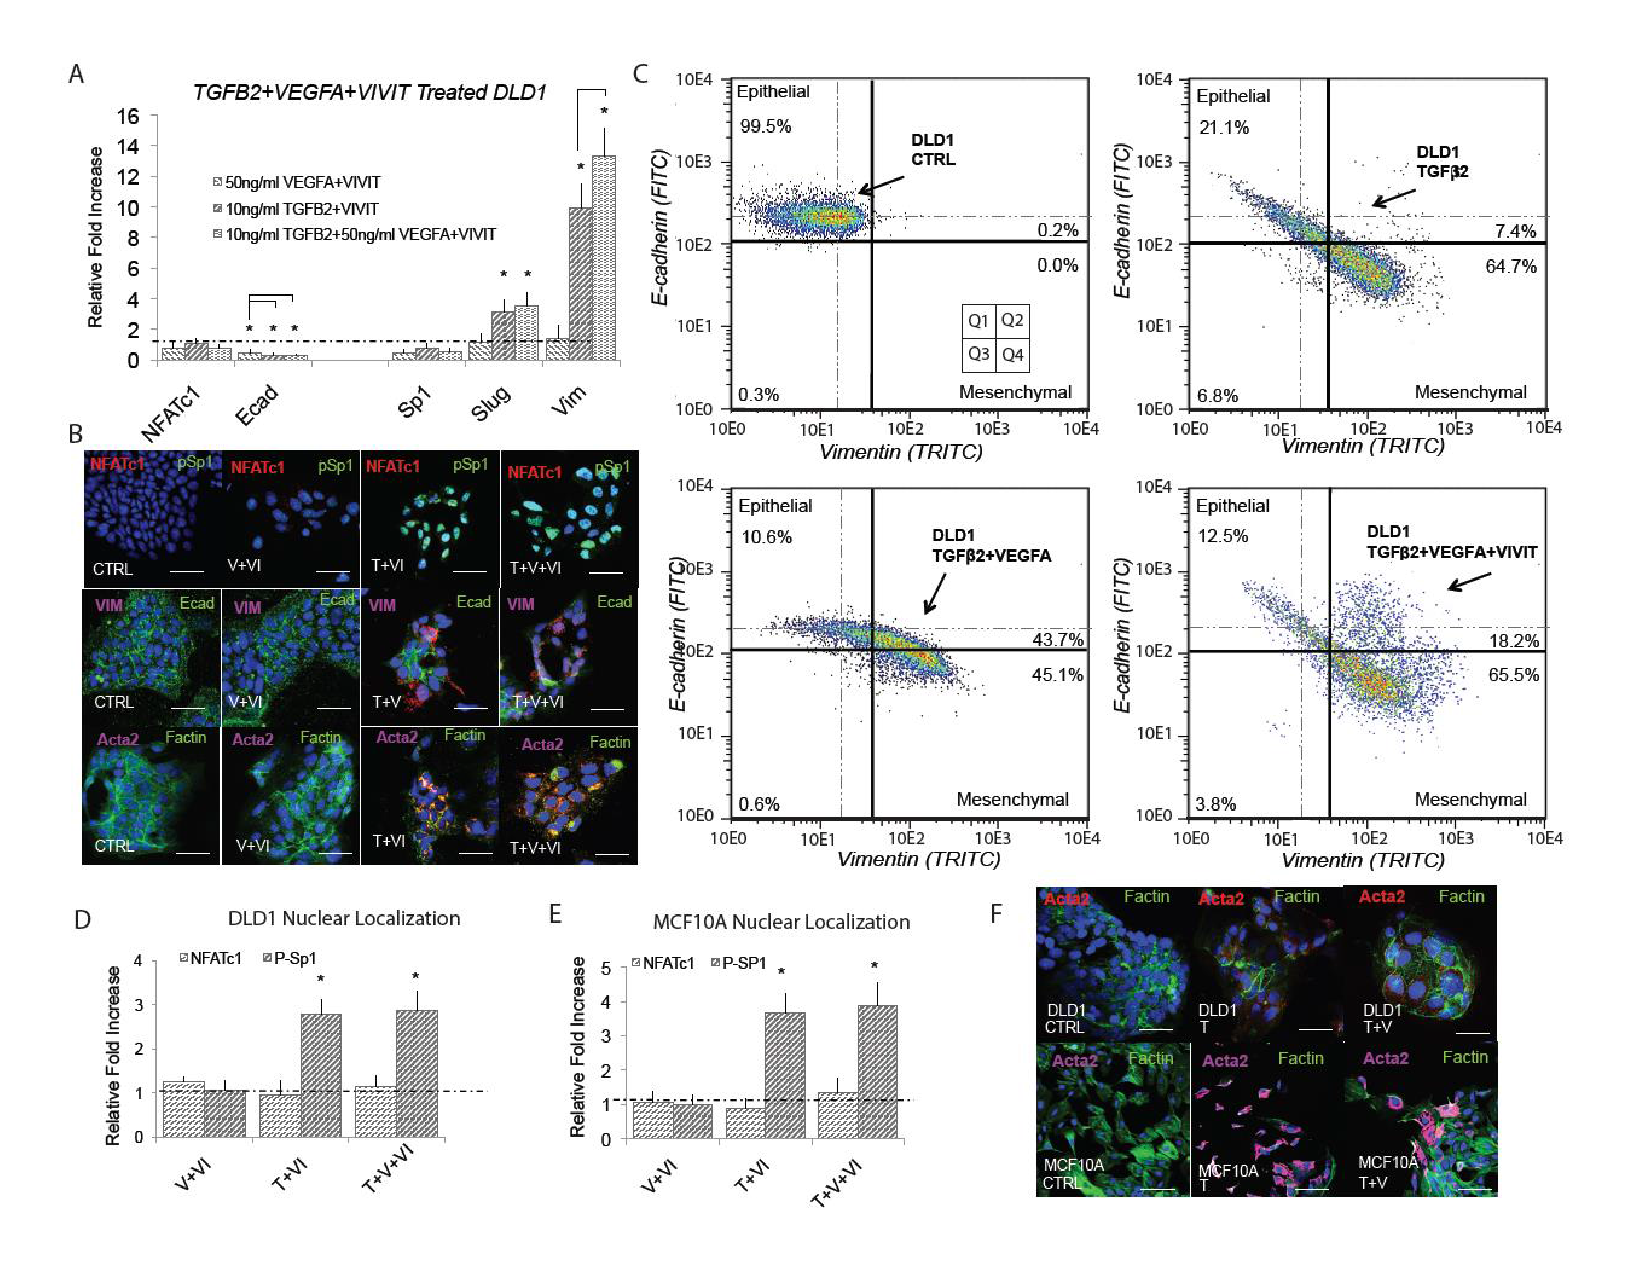
\includegraphics [width=1.0\linewidth] {./figs/Fig-4-Supplemental-DLD1-FlowCyto.pdf}
\caption{E-cadherin expression is dependent upon NFAT activity in DLD1.
(A) Treatment with VEGFA (50ng/ml) and NFAT inhibitory peptide VIVIT (10$\mu$M) resulted in significantly reduced ecadherin expression (qRT-PCR at 48hrs).
Addition of TGF$\beta$2 (10ng/ml) and VIVIT resulted in increased Slug and vimentin expression, while inhibiting ecadherin levels.
Combined TGF$\beta$2, VEGFA, and VIVIT treatment resulted in target genes Slug and vimentin expression increased, while inhibiting ecadherin levels.
No change in Sp1 or NFATc1 expression was found.
(B) These findings were confirmed via immunofluorescence as the VIVIT inhibitors was shown to inhibit ecadherin levels in all three cases.
We also found no change in gene or nuclear localization of NFATc1 in all three cases, while phospho-Sp1 was found to increase in both TGF$\beta$ conditions.
(C) Quantitative flow cytometry also confirmed this trend.
(D,E)  TGF$\beta$2, VEGFA and VIVIT treatment in DLD1 and MCF10A resulted in no change of Sp1 expression or NFATc1 expression.
(F)  Likewise, no change in nuclear localization of NFAT in all three cases, however phospho-Sp1 was found to increase in both TGF$\beta$ conditions.
Magnification, 40x. Scale bars: 50$\mu$m.  C=Control, T=TGF$\beta$2 , V=VEGFA, VI= NFAT inhibitor (VIVIT).
Asterisks signify statistical differences from each other according to a one-way ANOVA with Tukey's post hoc (p$\prec$0.05).}\label{fg:S4}
\end{figure}

\newpage

\begin{figure}
	\center
	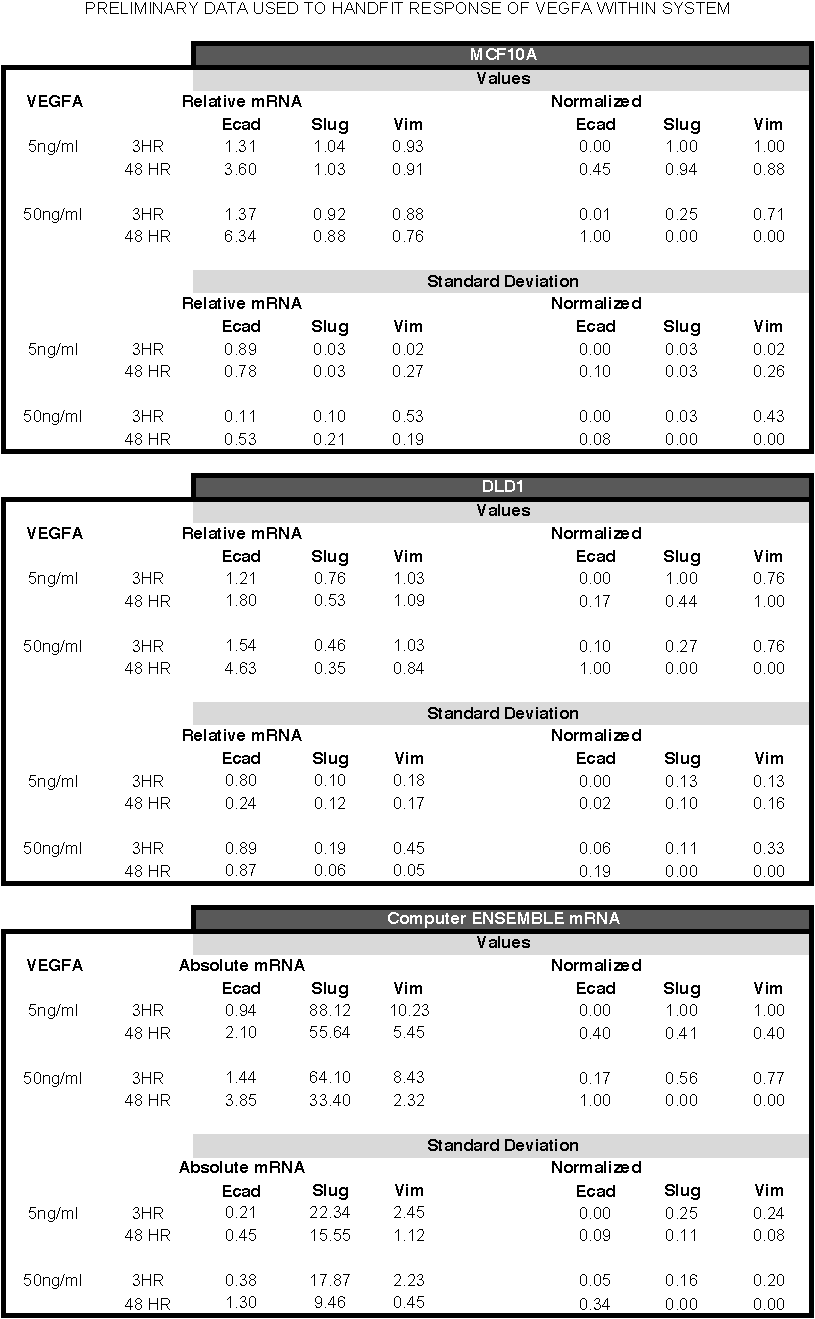
\includegraphics [width=0.75\linewidth] {./figs/Fig-Supplemental-Data-VEGFA.pdf}
	\caption{VEGF-A qPCR data used to hand fit VEGF enhancement of E-cadherin expression. mRNA was harvested after 3hr and 24hr timepoint.}\label{fg:VEGFA-Data}
\end{figure}


%\bibliography{References_v1}
